\documentclass[../analisi-dei-requisiti.tex]{subfiles}

\begin{document}%
\subsection{Attori}%
\label{subs:attori}

\subsubsection{Attori primari}%
\label{sssec:attori_primari}
\begin{description}
 \item \textbf{Utente}: Si fa riferimento all'utente che ha intenzione di effettuare l'analisi di un determinato dataset attraverso la \emph{exploratory data analysis (EDA)}.
\end{description}

\subsubsection{Attori secondari}
\label{sssec:attori_secondari}
\begin{description}
    \item \textbf{Database}: Fonte esterna dalla l'utente può effettuare query che ritorneranno i dati da visualizzare nei grafici.
\end{description}

\newpage
\subsection{UC1 - Creazione ambiente}
\label{sub:uc1}

%TODO: Add correct image
% Se uno use case esce dalla post allora non mettiamo in scenario secondario ma in estensione
% se invece la post rimane la stessa non è estensione.

\begin{figure}[h]
    \centering
    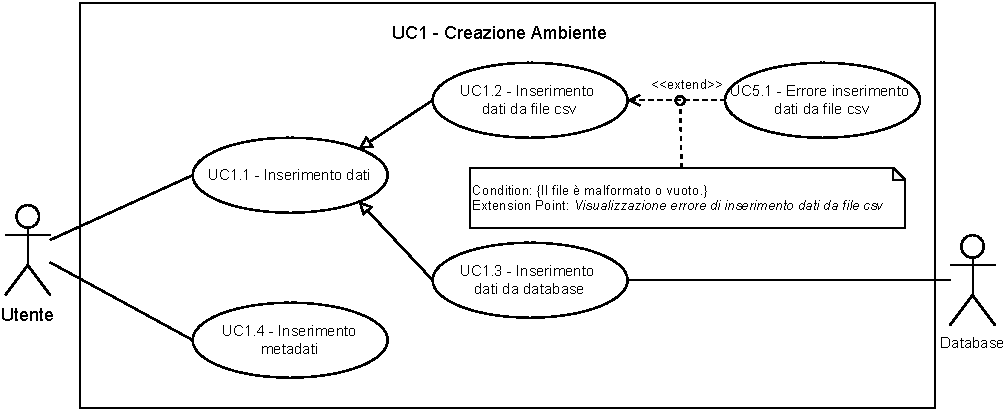
\includegraphics[width=0.7\textwidth]{componenti/casi-duso/diagrammi/UC1.pdf}
    \caption{Diagramma rappresentante UC1}
    \label{fig:UC1}
\end{figure}


\begin{itemize}
    \item \textbf{Descrizione}: L'utente prepara l'applicativo HDviz alla visualizzazione dei
                                dati importando un opportuno dataset e assegna, 
                                se non già definiti, dei metadati 
                                che descrivono il tipo del dato di ogni sua dimensione.
	
    \item \textbf{Attore primario}: Utente;
    \item \textbf{Attore secondario}: Database;
    
    
    \item \textbf{Precondizione}:   L'utente decide di caricare i dati.

    \item \textbf{Postcondizione}:  Viene caricato un dataset. 
    
                                    Ogni colonna del dataset ha associato
                                    un metatag che indica la tipologia della dimensione.

	\item \textbf{Scenario principale}:
		\begin{enumerate}
			\item L'utente seleziona l'opzione di aggiunta dei dati.
            \item L'utente seleziona la fonte dei dati da importare e li importa.
            \item Il dataset caricato è corretto e provvisto di validi metatag.
        \end{enumerate}
   
    \item \textbf{Scenario alternativo}:
		\begin{enumerate}
            \item Il dataset caricato presenta metadati non validi o ne è sprovvisto:
            \begin{enumerate}
                \item L'utente inserisce manualmente i metadati mancanti. (\hyperref[subsec:UC1.4]{UC1.4})
            \end{enumerate}
        \end{enumerate}

    \item \textbf{Generalizzazioni}:
    \begin{enumerate}
        \item Inserimento dati da file csv.
        \item Inserimento dati da database.
    \end{enumerate}
    
    \item \textbf{Estensioni}:
    \begin{enumerate}
        \item Se il caricamento da file fallise:
        \begin{enumerate}
            \item Il caricamento del dataset viene interrotto.
            \item Viene visualizzato un messaggio di errore. (UC5.1)
        \end{enumerate}
    \end{enumerate}
\end{itemize}

\subsubsection{UC1.1 - Inserimento dati}
\label{ssub:UC1.1}
\begin{itemize}
    \item \textbf{Descrizione}: L'utente decide di impostare l'ambiente creando un dataset i cui 
                                dati vengono caricati da file csv oppure da database al quale l'utente ha accesso.

    \item \textbf{Attore primario}: Utente.
    \item \textbf{Attore secondario}: Database;
    
    \item \textbf{Precondizione}:   L'utente decide di caricare i dati.

    \item \textbf{Postcondizione}:  Viene caricato un dataset non vuoto dalla fonte scelta dall'utente. 

	\item \textbf{Scenario principale}:
		\begin{enumerate}
			\item L'utente seleziona l'opzione di aggiunta dei dati:
            \begin{enumerate}
                \item L'utente sceglie di importare i dati da file (UC1.2)
                \item L'utente seleziona di importare i dati da database (UC1.3)
            \end{enumerate}
        \end{enumerate}

        \item \textbf{Generalizzazioni}:
        \begin{enumerate}
            \item Inserimento dati da file csv. (UC1.2)
            \item Inserimento dati da database. (UC1.3)
        \end{enumerate}
\end{itemize}


\subsubsection{UC1.2 - Inserimento dati da file csv}
\label{ssub:UC1.1.1}
\begin{itemize}
    \item \textbf{Descrizione}: L'utente importa un dataset non vuoto da un file csv del suo dispostivo.

    \item \textbf{Attore primario}: Utente.
    
    \item \textbf{Precondizione}:   L'utente selezione l'opzione di caricare i dati da un file csv.
    \item \textbf{Postcondizione}:  Viene caricato un dataset. 

	\item \textbf{Scenario principale}:
		\begin{enumerate}
			\item L'utente seleziona l'opzione di aggiunta dei dati mediante file.
			\item L'utente seleziona file di dati valido da importare.
        \end{enumerate}
     
    \item \textbf{Estensioni}
    \begin{enumerate}
    
        \item Se l'utente importa un file non valido oppure vuoto:
        \begin{enumerate}
            \item La creazione del dataset falllsice
            \item Viene visualizzato il messaggio di errore. (UC5.1.1)
        \end{enumerate}
    \end{enumerate}
\end{itemize}

\newpage
\begin{figure}[h]
    \centering
    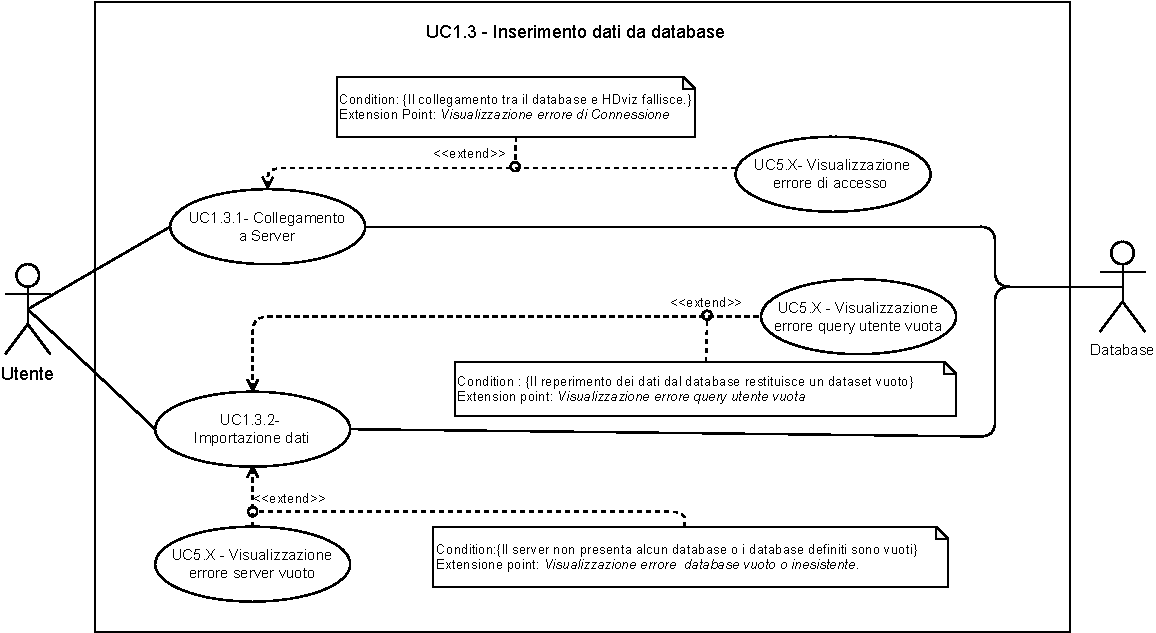
\includegraphics[width=0.9\textwidth]{componenti/casi-duso/diagrammi/UC1_3.pdf}
    \caption{Diagramma rappresentante UC1.3}
    \label{fig:UC1.3}
\end{figure}


\subsection{UC1.3 - Inserimento dati da database}
\label{ssub:UC1.3}
\begin{itemize}
    \item \textbf{Descrizione}: L'utente si connette ad un database di cui dispone accesso e 
                                crea un dataset non vuoto dal risultato di una ricerca delle tabelle che gli interessano
                                visualizzare successivamente in HDviz.
    \item \textbf{Attore primario}: Utente.
    
    \item \textbf{Attore secondario}: Database.
    
    \item \textbf{Precondizione}:   L'utente decide di caricare i dati mediante un database. 
    \item \textbf{Postcondizione}:  Viene caricato un dataset da un database. 

	\item \textbf{Scenario principale}:
		\begin{enumerate}
			\item L'utente effettua la connessione con un database da lui fornito. (UC1.3.1)
			\item L'utente importa i dati dal form di caricamento dati. (UC1.3.2)
        \end{enumerate}

    \item \textbf{Estensioni}:
    \begin{enumerate}
        \item Se l'apertura della connessione con il database fallisce.
        \begin{enumerate}
            \item L'inserimento dei dati viene interrotto.
            \item Viene visualizzato un messaggio di errore (UC5.2).
        \end{enumerate}

        \item Se il server al quale si è connessi non ha database o tutti sono vuoti.
        \begin{enumerate}
            \item L'inserimento dei dati viene interrotto.
            \item Viene visualizzato un messaggio di errore (UC5.3).
        \end{enumerate}

        \item Se la query utente è vuota:
        \begin{enumerate}
            \item L'inserimento dei dati viene interrotto.
            \item Viene visualizzato un messaggio di errore (UC5.4).
        \end{enumerate}
    \end{enumerate}
\end{itemize}


\newpage
\begin{figure}[h]
    \centering
    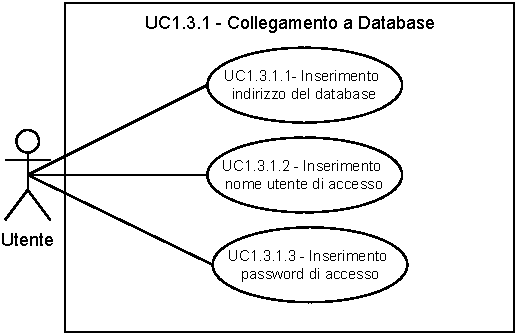
\includegraphics[width=0.5\textwidth]{componenti/casi-duso/diagrammi/UC1_3_1.pdf}
    \caption{Diagramma rappresentante UC1.3.1}
    \label{fig:UC1.3}
\end{figure}


\subsection{UC1.3.1 - Collegamento a Server}
\label{subsec:UC1.3.1}
\begin{itemize}
    \item \textbf{Descrizione}: L'utente apre una connessione con un server di dati del quale 
                                dispone le credenziali di accesso. 

    \item \textbf{Attore primario}: Utente.
    \item \textbf{Attore secondario}: Database.
    
    \item \textbf{Precondizione}:   L'utente decide di caricare i dati mediante un database.
    \item \textbf{Postcondizione}:  Viene aperta la connessione con un server di dati.

	\item \textbf{Scenario principale}:
		\begin{enumerate}
			\item L'utente immette i campi necessari per l'acceso: indirizzo, nome utente e password.
			\item HDviz si connette al server con i valori immessi dall'utente.
        \end{enumerate}
    \end{itemize}


\subsubsection{UC1.3.1.1 - Inserimento indirizzo}
\label{ssub:UC1.3.1.1}
\begin{itemize}
    \item \textbf{Descrizione}: L'utente inserisce l'indirizzo del server al quale vuole accedere.
    \item \textbf{Attore primario}: Utente.    
   
    \item \textbf{Precondizione}:   L'utente decide di caricare un dataset mediante un database.
    \item \textbf{Postcondizione}:  Viene inserito l'indirizzo del server di dati.
    
    \item \textbf{Scenario Principale}: L'utente inserisce l'indirizzo di connessione.

\end{itemize}


\subsubsection{UC1.3.1.2 - Inserimento nome utente}
\label{ssub:UC1.3.1.2}
\begin{itemize}
    \item \textbf{Descrizione}: L'utente inserisce il nome utente per accedere al server.
    \item \textbf{Attore primario}: Utente.
    
    \item \textbf{Precondizione}:   L'utente decide di caricare i dataset meidante un database.
    \item \textbf{Postcondizione}:  Viene inserito il nome utente per l'accessp al server di dati.

    \item \textbf{Scenario Principale}: L'utente inserisce il nome d'accesso.
\end{itemize}


\subsubsection{UC1.3.1.3 - Inserimento password}
\label{ssub:UC1.3.1.3}
\begin{itemize}
    \item \textbf{Descrizione}: L'utente inserisce la password per accedere al server.
    \item \textbf{Attore primario}: Utente.
    
    \item \textbf{Precondizione}:   L'utente decide di caricare i dataset meidante un database.
    \item \textbf{Postcondizione}:  Viene caricato un dataset dal database.

    \item \textbf{Scenario Principale}: L'utente inserisce la password d'accesso.

\end{itemize}

%TODO: Inserimento anche di database (non fa formalmente parte di una query)
\subsection{UC1.3.2 - Importazione dati}
\label{subsec:UC1.3.2}
\begin{itemize}
    \item \textbf{Descrizione}: L'utente ottiene i dati che da inserire nel nuovo dataset da un database
                                del server con cui ha una connessione aperta al momento, mediante 
                                l'esecuzione di una query personalizzata che fornisce in un form.

    \item \textbf{Attore primario}: Utente.
    
    \item \textbf{Attore secondario}: Database.
    
    \item \textbf{Precondizione}:   L'utente ha aperto una connessione con un server dati.
    \item \textbf{Postcondizione}:  Viene costruito il dataset dai dati reperiti dall'utente mediante un file di query.

	\item \textbf{Scenario principale}:
        \begin{enumerate}
            \item L'utente seleziona il database del server sul quale fare la selezione.
			\item L'utente inserisce nel form una query per il riperimento dei dati che viene eseguita sul server.
			\item Viene costruito il dataset dal risultato della ricerca.
        \end{enumerate}
    %TODO CApire dove diamine vanno messe le estensioni.
\end{itemize}






\subsection{UC1.4 - Inserimento metadati}
\label{subsec:UC1.4}
\begin{itemize}
    \item \textbf{Descrizione}: L'utente assegna ad ogni colonna del dataset importato,
                                in cui non è già correttamente definito,
                                dei metatag che ne descrivono le proprietà.


    \item \textbf{Attore primario}: Utente.
    
    \item \textbf{Precondizione}:   L'utente ha caricato un dataset e non tutti i suoi metadati sono validi o definiti.
    \item \textbf{Postcondizione}:  Il dataset caricato è provvisto di metadati validi. 

	\item \textbf{Scenario principale}:
		\begin{enumerate}
            \item L'utente assegna ad ogni colonna del dataset il tipo di dato che rappresenta (metatag) scegliendo tra:
                    Nominale, Ordinale, Intervallo o Rapporto.
        \end{enumerate}

\end{itemize}


\newpage
\newpage

\subsection{UC2 - Creazione di un grafico}
\label{sub:uc2}

%TODO: Add correct image
\begin{figure}[h]
    \centering
    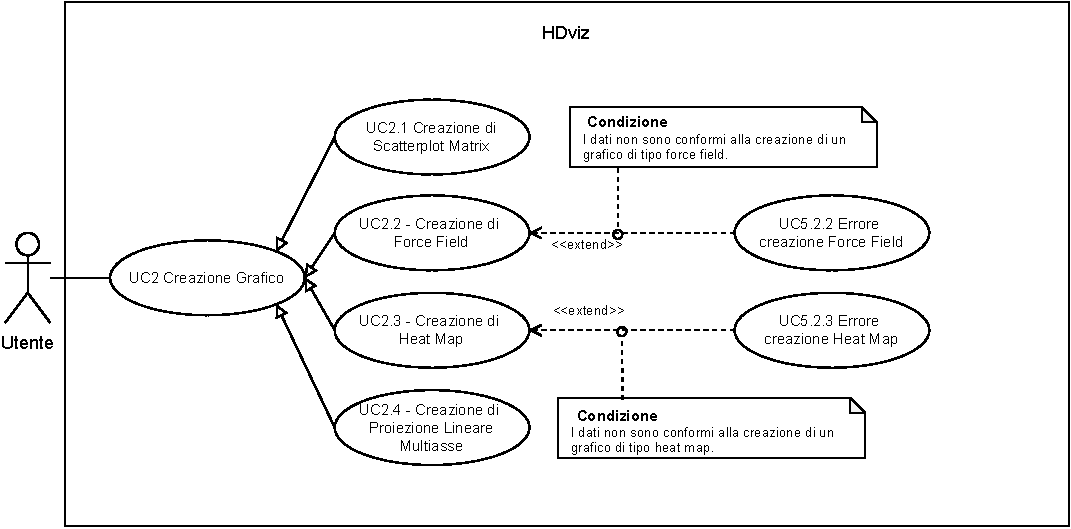
\includegraphics[width=0.8\textwidth]{componenti/casi-duso/diagrammi/UC2.pdf}
    \caption{Diagramma rappresentante UC2}
    \label{fig:UC2}
\end{figure}


\begin{itemize}
    \item \textbf{Descrizione}: L’utente vuole procedere con la fase di esplorazione
                                dati mediante la visualizzazione del dataset
                                attraverso uno dei diversi grafici proposti dall’applicativo
                                che ne costruisce uno e lo visualizza.
	
    \item \textbf{Attore primario}: Utente;
    
    \item \textbf{Precondizione}:   Nella sessione è stato importato un dataset e ogni 
                                    suo campo ha un metatag associato.

    \item \textbf{Postcondizione}:  Viene calcolato il grafico della tipologia scelta dai dati 
									dal dataset importato dotato di metatag validi e successivamente 
									visualizzato all'utente.

	\item \textbf{Scenario principale}:
		\begin{enumerate}
			\item L'utente seleziona l'opzione che desidera tra le tipologie di grafico.
			\item HDviz visualizza il grafico ottenuto dalla costruzione dei dati.
        \end{enumerate}

    \item \textbf{Generalizzazioni:}:  L'utente seleziona il grafico desiderato tra:

    \begin{enumerate}
        
        \item Grafico scatterplot matrix (UC2.1).
        \item Grafico force field (UC2.2).
        \item Grafico heat map (UC2.3).
        \item Grafico proiezione lineare multiasse (UC2.4).
        
	\end{enumerate}

\end{itemize}

% TODO: Make error for each selected graph type.
\subsubsection{UC2.1 Selezione di Scatterplot matrix}
\label{ssub:UC2.1}
\begin{itemize}

    \item \textbf{Attore primario}: Utente;

    \item \textbf{Precondizione}:   Un dataset è stato correttamente importato e ad ogni campo ha associato
                                    un metatag valido;

    \item \textbf{Postcondizione}:  Viene calcolato il grafico di tipo Scatterplot Matrix;

	\item \textbf{Scenario Principale}: HDviz costruisce un grafico Scatterplot matrix con il dataset 
										importato.
\end{itemize}


\subsubsection{UC2.2 Selezione di Force Field}
\label{ssub:UC2.2}
\begin{itemize}

    \item \textbf{Attore primario}: Utente;

    \item \textbf{Precondizione}:   Un dataset è stato correttamente importato e ad ogni campo ha associato
                                    un metatag valido;

    \item \textbf{Postcondizione}:  Viene calcolato il grafico di tipo Force Field;
	
	\item \textbf{Scenario Principale}: HDviz costruisce un grafico Force Field con il dataset importato.
	% Secondo me fa in scenario alternativo e in estensione solo lo UC a cui si riferisce. Pensaci
	% I pro apes fanno tutto in estensioni mentre i Qbeam fanno scenario alternativo e mettono in estensione solo UC riferimento
	\item \textbf{Estensioni}:
	\begin{enumerate}
		\item Se il dataset corrente non è compatibile con il grafico di tipo Force Field:
		\begin{enumerate}
			\item La costruzione del grafico fallisce.
			\item Viene visualizzato un messaggio di errore. (UC4.2.2)
		\end{enumerate}
	\end{enumerate}
\end{itemize}


\subsubsection{UC2.3 Selezione di Heat Map}
\label{ssub:UC2.3}
\begin{itemize}

    \item \textbf{Attore primario}: Utente;

	\item \textbf{Precondizione}:   Un dataset è stato correttamente importato e ad ogni campo 
									ha associato un metatag;

    \item \textbf{Postcondizione}:  Viene calcolato il grafico di tipo Heat map dal progetto corrente
	\item \textbf{Scenario Principale}: HDviz costruisce un grafico Heat Map con il dataset importato.
	% Secondo me fa in scenario alternativo e in estensione solo lo UC a cui si riferisce. Pensaci
	% I pro apes fanno tutto in estensioni mentre i Qbeam fanno scenario alternativo e mettono in estensione solo UC riferimento
	\item \textbf{Estensioni}:
	\begin{enumerate}
		\item Se il dataset corrente non è compatibile con il grafico di tipo Heat Map:
		\begin{enumerate}
			\item La costruzione del grafico fallisce.
			\item Viene visualizzato un messaggio di errore. (UC4.2.3)
		\end{enumerate}
	\end{enumerate}
\end{itemize}


\subsubsection{UC2.4 Selezione di Proiezione Lineare Multiasse}
\label{ssub:UC2.4}
\begin{itemize}

    \item \textbf{Attore primario}: Utente;

    \item \textbf{Precondizione}:   Un dataset è stato correttamente importato e ad ogni campo ha associato
                                    un metatag;

    \item \textbf{Postcondizione}:  Viene calcolato il grafico di tipo \emph{"Proiezione lineare multiasse"} dal progetto corrente

	\item \textbf{Scenario Principale}: HDviz costruisce un grafico Proiezione Lineare Multiasse con il dataset importato.
\end{itemize}

\subsubsection{UC2.5 Selezione di Distance Map}
\label{ssub:UC2.5}
\begin{itemize}
	\item \textbf{Descrizione}:			Viene selezionata la visualizzazione dei dati mediante graafico \emph{Distance Map}
	\item \textbf{Attore primario}:		Utente;
	\item \textbf{Precondizione}:		È stato importato correttamente un dataset (UC1 \refSec{subsec:uc1})
	\item \textbf{Postcondizione}:		É stato selezionata la visualizzazione del grafico \emph{Distance Map} con i dati 
										precedentemente importati
	
	\item \textbf{Scenario Principale}: L'utente seleziona il grafico \emph{Distance Map} tra le opzioni proposte
\end{itemize}
\newpage
\newpage
\subsection{UC3 - Modifica Metadati}
\label{subsec:uc3}

\begin{figure}[h]
    \centering
    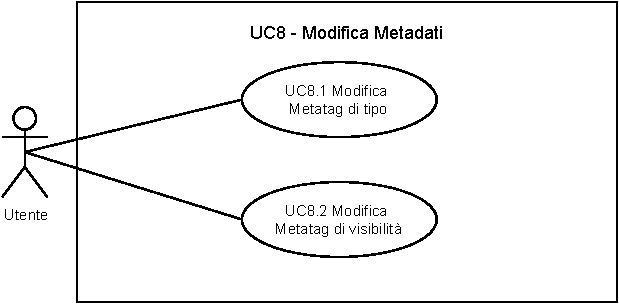
\includegraphics[width=0.7\textwidth]{componenti/casi-duso/diagrammi/UC3.pdf}
    \caption{Diagramma rappresentante UC3}
    \label{fig:UC3}
\end{figure}

\begin{itemize}
    \item \textbf{Descrizione}: L’utente vuole modificare uno o più metadati attualmente assegnati al dataset.
	
    \item \textbf{Attore primario}: Utente.
    
    \item \textbf{Precondizione}:   Nel programma è stato importato un dataset dotato di metadati per ogni sua colonna.
    \item \textbf{Postcondizione}:  Vengono aggiornati i metadati del dataset se modificati.

	\item \textbf{Scenario principale}:
		\begin{enumerate}
			\item L'utente decide se effettuare modifiche ai metatag e le effettua.
			\item L'utente effettua modifiche che ritiene necessarie tra quelle possibili.
			\item L'utente conferma le modifiche premendo il pulsante di conferma.
        \end{enumerate}

    %TODO: Riprisino è comunque un aggiornamento giusto? Dovremmo mettere un'estensione?
    \item \textbf{Scenario alternativo}:
		\begin{enumerate}
			\item L'utente decide di annullare le modifiche.
			\item Vengono ripristinati i metatag precedenti alla modifica.
        \end{enumerate}
\end{itemize}
\newpage
\subsubsection{UC3.1 - Modifica metadati di tipo}
\label{subsubsec:uc3.1}

\begin{itemize}
    \item \textbf{Descrizione}: L’utente vuole modificare uno o più metatag di tipo attualmente assegnati alle dimensioni del dataset.
	
    \item \textbf{Attore primario}: Utente.
    
    \item \textbf{Precondizione}:   Nel programma è stato importato un dataset dotato di metadati per 
                                    ogni sua colonna e l'utene seleziona la voce di modifica dei metatag di tipo.
    \item \textbf{Postcondizione}:  Vengono aggiornati i metatag di tipo del dataset che sono stati modificati.

	\item \textbf{Scenario principale}:
		\begin{enumerate}
            \item L'utente seleziona le dimensioni del dataset che vuole modificare.
            \item L'utente modifica il tipo di metatag di ogni dimensione selezionata.
        \end{enumerate}
\end{itemize}


\subsubsection{UC3.2 - Modifica metatag di visibilità}
\label{subsubsec:uc3.2}

\begin{itemize}
    \item \textbf{Descrizione}: L’utente vuole modificare uno o più metatag di visibilità attualmente assegnati al dataset.
	
    \item \textbf{Attore primario}: Utente.
    
    \item \textbf{Precondizione}:   Nel programma è stato importato un dataset dotato di metadati per 
                                    ogni sua colonna e l'utene seleziona la voce di modifica dei metatag di visibilità.
    \item \textbf{Postcondizione}:  Vengono aggiornati i metatag di visibilità del dataset che sono stati modificati.

	\item \textbf{Scenario principale}:
		\begin{enumerate}
            \item L'utente seleziona le dimensioni del dataset che vuole modificare.
            \item L'utente decide se rendere visibile o meno le dimensioni selezionate.
        \end{enumerate}
\end{itemize}


\newpage
\newpage
\subsection{UC4 - Modifica Grafico}
\label{subsec:uc4}

%TODO: Add correct image
\begin{figure}[h]
    \centering
    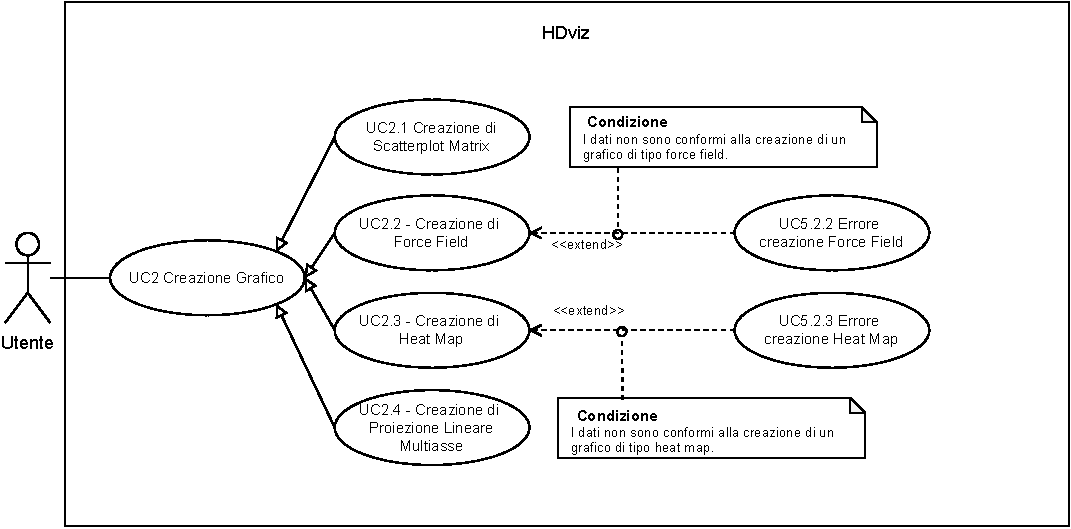
\includegraphics[width=0.8\textwidth]{componenti/casi-duso/diagrammi/UC2.pdf}
    \caption{Diagramma rappresentante UC2}
    \label{fig:UC4}
\end{figure}


\begin{itemize}
    \item \textbf{Descrizione}: L’utente modifica la visualizzazione del grafico precedentemente costruito
                                e ne vede le modifiche.
	
    \item \textbf{Attore primario}: Utente.
    
    \item \textbf{Precondizione}:   Nel programma è stato importato un dataset dotato di metatag per ogni
                                    colonna dei dati ed è stato costruito un grafico di una tipologia scelta dall'utente.

    \item \textbf{Postcondizione}:  Viene aggiornato il grafico costruito e visualizzato con i nuovi parametri.

	\item \textbf{Scenario principale}:
		\begin{enumerate}
			\item L'utente decide di modificare il grafico corrente.
			\item L'utente effettua le modifiche desiderate.
            \item L'utente conferma le modifiche apportate selezionando il pulsante di conferma.
        \end{enumerate}

    \item \textbf{Scenario alternativo}:
        \begin{enumerate}
            \item L'utente decide di annullare le modifiche effettuate (UC4.5) al posto di confermarle.   
            \item Le modifiche vengono scartate e viene ripristinata la visualizzazione del grafico prima delle modifiche.
        \end{enumerate}
    
\end{itemize}


\subsection{UC4.1 Modifica Scatterplot Matrix}
\label{subsec:uc4.1}

\begin{figure}[h]
    \centering
    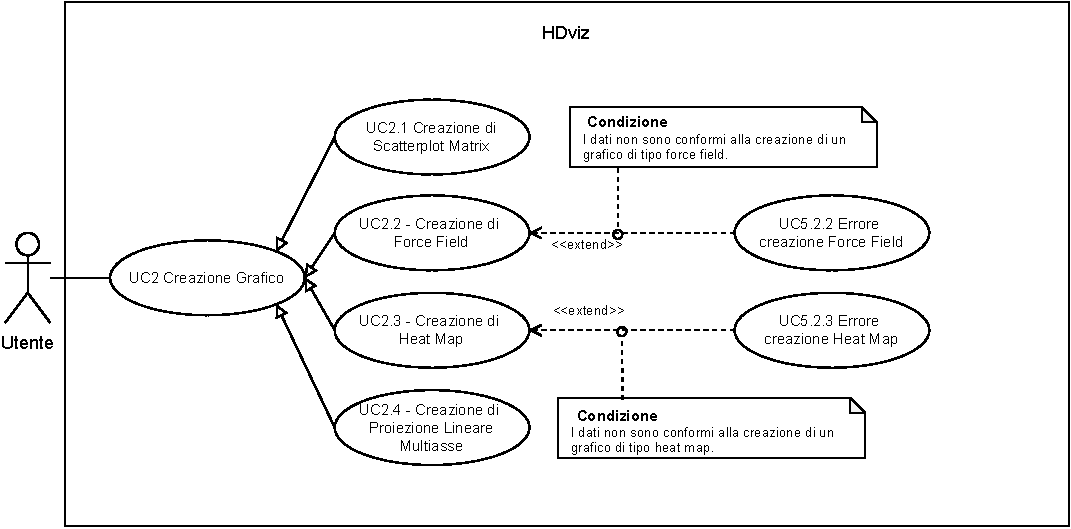
\includegraphics[width=0.8\textwidth]{componenti/casi-duso/diagrammi/UC2.pdf}
    \caption{Diagramma rappresentante UC2}
    \label{fig:UC2}
\end{figure}


\begin{itemize}
    \item \textbf{Descrizione}: L’utente vuole modificare la visualizzazione dello Scatterplot Matrix
                                costruito dal dataset corrente.
	
    \item \textbf{Attore primario}: Utente.
    
    \item \textbf{Precondizione}:   Il grafico precedentemente costruito dal dataset corrente è uno Scatterplot Matrix.

    \item \textbf{Postcondizione}:  Viene aggiornato il grafico costruito e visualizzato con i nuovi parametri.

	\item \textbf{Scenario principale}:
		\begin{enumerate}
            \item L'utente apporta le modifiche desiderate tra quelle offerte dallo Scatterplot Matrix.
        \end{enumerate}
\end{itemize}


\subsubsection{UC4.1.1 Selezione dimensioni del grafico}
\label{subsec:uc4.1.1}
\begin{itemize}
    \item \textbf{Descrizione}: L’utente dispone di dati con metadati assegnati e può 
                                scegliere fino a 5 dimensioni che possono essere visualizzate nello Scatterplot Matrix.
	
    \item \textbf{Attore primario}: Utente.
    
    \item \textbf{Precondizione}:   Il grafico precedentemente costruito dal dataset corrente è uno Scatterplot Matrix.
    \item \textbf{Postcondizione}:  Vengono modificate le dimensioni visualizzate nei plot dello Scatterplot Matrix.

	\item \textbf{Scenario principale}:
        \begin{enumerate}
            \item L'utente seleziona l'opzione di selezione delle dimensioni.
            \item L'utente seleziona fino a cinque dimensioni scartandone una ogni volta.
            \item La visualizzazione sostituisce le dimensioni scartate con le nuove selezionate.
        \end{enumerate}
\end{itemize}


\subsubsection{UC4.1.2 Selezione punto all'interno del grafico}
\label{subsec:uc4.1.1}
\begin{itemize}
    \item \textbf{Descrizione}: L'utente seleziona un punto in uno scatterplot della Matrice per vedere come 
                                esso viene rappresentato negli altri grafici a dispersione.
	
    \item \textbf{Attore primario}: Utente.
    
    \item \textbf{Precondizione}:   Il grafico precedentemente costruito dal dataset corrente è uno Scatterplot Matrix.
    \item \textbf{Postcondizione}:  Le proiezioni del punto selezionato, se appartentente allo Scatterplot, 
                                    venogno evidenziate in tutti i grafici della visualizzazione.

	\item \textbf{Scenario principale}:
        \begin{enumerate}
            \item L'utente seleziona un punto contente un vertice dello Scatterplot.
            \item La proiezione del punto viene evidenziata in tutti i diversi Scatterplot della visualizzazione.
        \end{enumerate}

    \item \textbf{Scenario alternativo}:
        \begin{enumerate}
            \item Se l'utente seleziona un punto vuoto dello Scatterplot la visualizzazione non evidenzia alcun punto del grafico.
        \end{enumerate}

\end{itemize}


\subsubsection{UC4.1.3 Selezione di un insieme di punti del grafico}
\label{subsec:uc4.1.1}
\begin{itemize}
    \item \textbf{Descrizione}: L'utente seleziona un insieme di punti in uno scatterplot della Matrice per vedere come 
                                essi vengono rappresentati negli altri grafici a dispersione.
	
    \item \textbf{Attore primario}: Utente.
    
    \item \textbf{Precondizione}:   Il grafico precedentemente costruito dal dataset corrente è uno Scatterplot Matrix.
    \item \textbf{Postcondizione}:  Le proiezioni dei punti selezionati, se appartentente allo Scatterplot, 
                                    vengono evidenziate in tutti i grafici della visualizzazione.

	\item \textbf{Scenario principale}:
        \begin{enumerate}
            \item L'utente seleziona un'aerea di punti di uno Scatterplot della matrice.
            \item Le proiezioni dei punti vengono evidenziate in tutti i diversi Scatterplot della visualizzazione.
        \end{enumerate}

    \item \textbf{Scenario alternativo}:
        \begin{enumerate}
            \item Se l'utente seleziona un'area di punti vuota dello Scatterplot la visualizzazione non evidenzia alcun punto della matrice.
        \end{enumerate}

\end{itemize}





\subsection{UC4.2 Modifica Force Field}
\label{subsec:uc4.2}
% TODO: Create image for force field graph.
\begin{figure}[h]
    \centering
    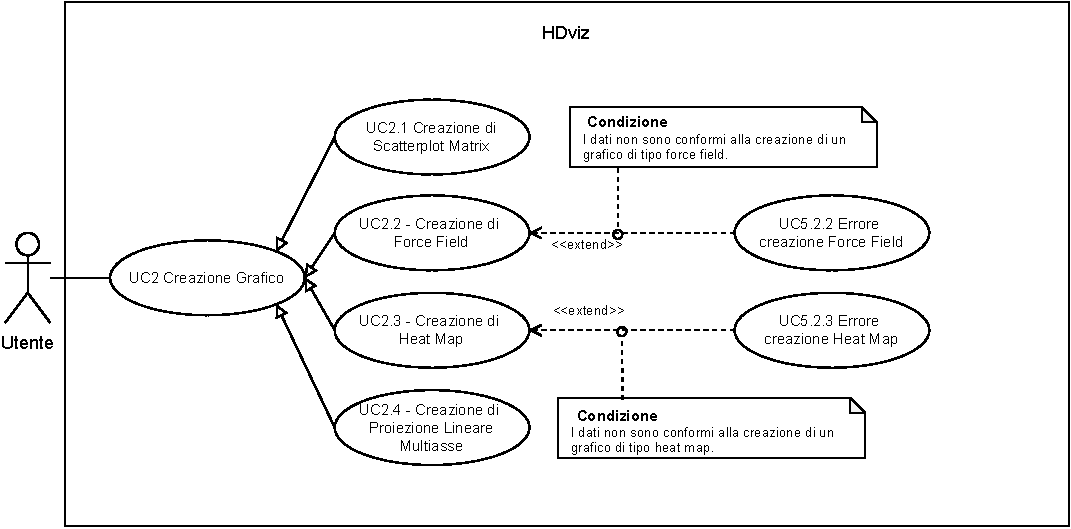
\includegraphics[width=0.8\textwidth]{componenti/casi-duso/diagrammi/UC2.pdf}
    \caption{Diagramma rappresentante UC2}
    \label{fig:UC2}
\end{figure}


\begin{itemize}
    \item \textbf{Descrizione}: L’utente vuole modificare la visualizzazione del grafo Force Field
                                costruito dal dataset corrente.
	
    \item \textbf{Attore primario}: Utente.
    
    \item \textbf{Precondizione}:   Il grafico precedentemente costruito dal dataset corrente è un Force Field.

    \item \textbf{Postcondizione}:  Viene aggiornato il grafico costruito e visualizzato con i nuovi parametri.

	\item \textbf{Scenario principale}:
		\begin{enumerate}
            \item L'utente apporta le modifiche desiderate tra quelle offerte dal Force Field.
        \end{enumerate}
\end{itemize}

\subsubsection{UC4.2.1 Modifica posizione dei nodi}
\label{subsec:uc4.2.1}
\begin{itemize}
    \item \textbf{Descrizione}: L’utente vuole esplorare meglio i dati e decide di 
                                modificare la posizione dei nodi del grafo, trascinandoli con il 
                                cursore nell'area definita dal grafico.
	
    \item \textbf{Attore primario}: Utente.
    
    \item \textbf{Precondizione}:   Il grafico precedentemente costruito dal dataset corrente è un Force Field.
    \item \textbf{Postcondizione}:  Viene modificata la posizione dei nodi del grafo nella visualizzazione.

	\item \textbf{Scenario principale}:
        \begin{enumerate}
            \item L'utente tiene premuto il tasto di selezione e trascina il cursore sponstando il nodo nello spazio della visualizzazione.
            \item La visualizzazione muove i punti del grafo mantentendo le connessioni tra i nodi.
        \end{enumerate}
\end{itemize}

\subsubsection{UC4.2.2 Modifica dell'algoritmo delle distanze}
\label{subsec:uc4.2.2}
\begin{itemize}
    \item \textbf{Descrizione}: L’utente decide di cambiare l’algoritmo usato per il calcolo delle distanze.

	
    \item \textbf{Attore primario}: Utente.
    
    \item \textbf{Precondizione}:   Il grafico precedentemente costruito dal dataset corrente è un Force Field.
    \item \textbf{Postcondizione}:  Viene modificata la distanza tra i nodi del grafo nella visualizzazione.

	\item \textbf{Scenario principale}:
        \begin{enumerate}
            \item L'utente seleziona il menu delle distanze e seleziona uno degli algoritmi presentati nel menù.
            \item La visualizzazione modifica la distanza tra i nodi secondo l'algoritmo scelto.
        \end{enumerate}
\end{itemize}

\subsubsection{UC4.2.3 Modifica intensità forza attrattiva tra nodi}
\label{subsec:uc4.2.3}
\begin{itemize}
    \item \textbf{Descrizione}: Per poter visualizzare meglio i cluster di dati l’utente 
                                decide di scalare la forza di attrattiva tra i nodi.

	
    \item \textbf{Attore primario}: Utente.
    
    \item \textbf{Precondizione}:   Il grafico precedentemente costruito dal dataset corrente è un Force Field.
    \item \textbf{Postcondizione}:  Viene modificata l'intensità della forza attrattiva tra i nodi del grafo nella visualizzazione.

	\item \textbf{Scenario principale}:
        \begin{enumerate}
            \item L'utente seleziona la barra intensità e trascinando il cursore sulla barra varia l’intensità.
            \item La visualizzazione modifica l'intensità della forza secondo il valore selezionato nel grafo.
        \end{enumerate}
\end{itemize}

\subsubsection{UC4.2.4 Modifica proprietà di un nodo per dimensione}
\label{subsec:uc4.2.4}
\begin{itemize}
    \item \textbf{Descrizione}: Per poter visualizzare meglio i cluster di dati l’utente 
                                decide di scalare la forza di attrattiva tra i nodi.

	
    \item \textbf{Attore primario}: Utente.
    
    \item \textbf{Precondizione}:   Il grafico precedentemente costruito dal dataset corrente è un Force Field.

    \item \textbf{Postcondizione}:  Viene modificato lo stile dei nodi per una determinata dimensione del grafo costruito.

	\item \textbf{Scenario principale}:
        \begin{enumerate}
        
            \item L'utente seleziona il menu delle dimensioni.
            \item L'utente seleziona la dimensione di interesse.
            \item L'utente manipola le proprietà che gli interessano.
            \item La visualizzazione mostra i nuovi nodi per la dimensione selezionata.
                
        \end{enumerate}
\end{itemize}


\subsubsection{UC4.2.4.1 Modifica colore}
\label{subsec:uc4.2.4.1}
\begin{itemize}
    \item \textbf{Descrizione}: L'utente decide di modificare il colore di nodi relativi ad una dimensione.

	
    \item \textbf{Attore primario}: Utente.
    
    \item \textbf{Precondizione}:   L'utente ha selezionato l'opzione di modifica delle proprietà dei nodi per dimensione (UC4.2.4).
    \item \textbf{Postcondizione}:  Viene aggiornato il colore dei nodi della dimensione selezionata.

	\item \textbf{Scenario principale}:
        \begin{enumerate}
            \item L'utente seleziona il nuovo colore da assegnare ai nodi tra quelli resi disponbili.
        \end{enumerate}
\end{itemize}

\subsubsection{UC4.2.4.2 Modifica raggio}
\label{subsec:uc4.2.2}
\begin{itemize}
    \item \textbf{Descrizione}: L'utente decide di modificare il raggio di nodi relativi ad una dimensione.
	
    \item \textbf{Attore primario}: Utente.
    
    \item \textbf{Precondizione}:   L'utente ha selezionato l'opzione di modifica delle proprietà dei nodi per dimensione (UC4.2.4).
    \item \textbf{Postcondizione}:  Viene aggiornato il raggio dei nodi della dimensione selezionata.

	\item \textbf{Scenario principale}:
        \begin{enumerate}
            \item L'utente fa variare il raggio dei nodi mediante uno slider.
        \end{enumerate}
\end{itemize}

\subsubsection{UC4.2.4.3 Modifica opacità}
\label{subsec:uc4.2.3}
\begin{itemize}
    \item \textbf{Descrizione}:  L'utente decide di modificare l'opacità dei nodi relativi ad una dimensione.

	
    \item \textbf{Attore primario}: Utente.

    \item \textbf{Precondizione}: L'utente ha selezionato l'opzione di modifica delle proprietà dei nodi per dimensione (UC4.2.4).
    \item \textbf{Postcondizione}:  Viene aggiornata l'opacità dei nodi della dimensione selezionata.

	\item \textbf{Scenario principale}:
        \begin{enumerate}
            \item L'utente fa variare l'opacità dei nodi mediante uno slider.
        \end{enumerate}
\end{itemize}

%%  _________________________
%
%%  Sezione della Heat Map
%%  _________________________

\subsection{UC4.3 Modifica Heat Map}
\label{subsec:uc4.3}
% TODO: Create image for force field graph.
\begin{figure}[h]
    \centering
    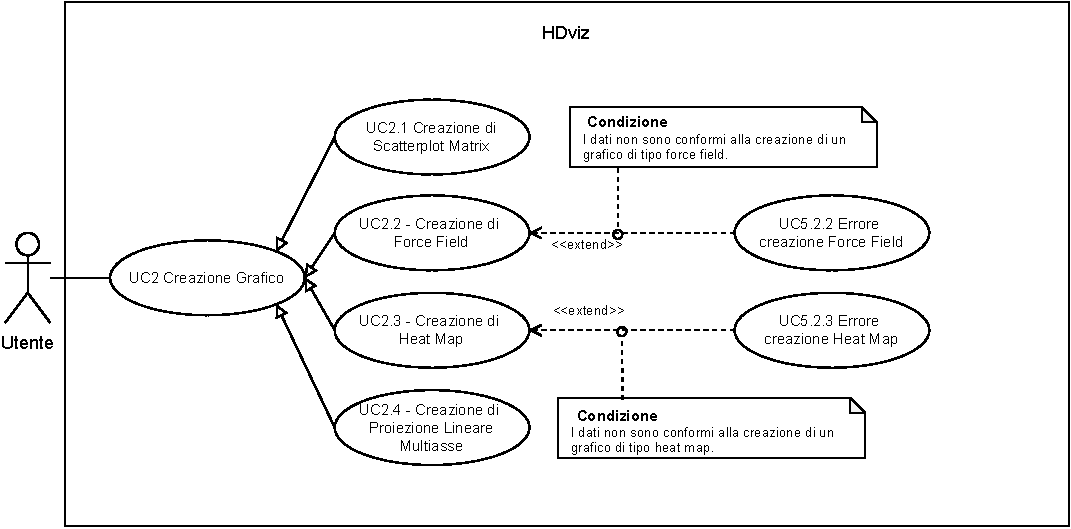
\includegraphics[width=0.8\textwidth]{componenti/casi-duso/diagrammi/UC2.pdf}
    \caption{Diagramma rappresentante UC2}
    \label{fig:UC2}
\end{figure}


\begin{itemize}
    \item \textbf{Descrizione}: L’utente vuole modificare la visualizzazione della Heat Map
                                costruita dal dataset corrente.
	
    \item \textbf{Attore primario}: Utente.
    
    \item \textbf{Precondizione}:   La visualizzazione costruita dal dataset corrente è un grafico di tipo Heat Map.

    \item \textbf{Postcondizione}:  Viene aggiornato il grafico costruito e visualizzato con i nuovi parametri.

	\item \textbf{Scenario principale}:
		\begin{enumerate}
            \item L'utente apporta le modifiche desiderate tra quelle offerte dalla Heat Map.
        \end{enumerate}
\end{itemize}

\subsubsection{UC4.3.1 Modifica scala dei colori}
\label{subsec:uc4.2.1}
\begin{itemize}
    \item \textbf{Descrizione}: L’utente vuole esplorare meglio i dati e decide di 
                                modificare la scala dei colori applicata alla Heat Map scegliendo una 
                                tra quelle proposte.
	
    \item \textbf{Attore primario}: Utente.
    
    \item \textbf{Precondizione}:   La visualizzazione costruita dal dataset corrente è una Heat Map.
    \item \textbf{Postcondizione}:  Viene modificata la scala dei colori del grafico nella visualizzazione.

	\item \textbf{Scenario principale}:
        \begin{enumerate}
            \item L'utente seleziona la voce "Scala dei colori" e seleziona una delle opzioni disponibili.
            \item La visualizzazione cambia la scala dei colori adottata dalla Heat Map.
        \end{enumerate}
\end{itemize}

\subsubsection{UC4.3.2 Applicare ordinamento alle righe}
\label{subsec:uc4.2.1}
\begin{itemize}
    \item \textbf{Descrizione}: L’utente per esplorare meglio i dati decide di ordinare le righe della Heat Map
                                seguendo l'algortimo di clustering gerarchico il quale aggiunge un dendogramma alla visualizzazione corrente.
	
    \item \textbf{Attore primario}: Utente.
    
    \item \textbf{Precondizione}:   La visualizzazione costruita dal dataset corrente è una Heat Map.
    \item \textbf{Postcondizione}:  Le righe della Heat Map vengono visualizzati secondo l'ordine imposto dall'algoritmo di ordinamento.

	\item \textbf{Scenario principale}:
        \begin{enumerate}
            \item   L'utente seleziona la casella di ordinamento delle righe.
            \item   La visualizzazione aggiorna l'ordinamento delle righe della Heat Map e viene aggiunto 
                    il dendogramma relativo alle righe.
        \end{enumerate}
\end{itemize}

\subsubsection{UC4.3.3 Applicare ordinamento alle colonne}
\label{subsec:uc4.2.1}
\begin{itemize}
    \item \textbf{Descrizione}: L’utente per esplorare meglio i dati decide di ordinare le colonne della Heat Map
                                seguendo l'algortimo di clustering gerarchico il quale aggiunge un dendogramma alla visualizzazione corrente.
	
    \item \textbf{Attore primario}: Utente.
    
    \item \textbf{Precondizione}:   La visualizzazione costruita dal dataset corrente è una Heat Map..
    \item \textbf{Postcondizione}:  Le colonne della Heat Map vengono visualizzati secondo l'ordine imposto dall'algoritmo di ordinamento.

	\item \textbf{Scenario principale}:
        \begin{enumerate}
            \item   L'utente seleziona la casella di ordinamento delle colonne.
            \item   La visualizzazione aggiorna l'ordinamento delle colonne della Heat Map 
                    e viene aggiunto il dendogramma relativo alle righe.
        \end{enumerate}
\end{itemize}


\subsubsection{UC4.3.4 Impostazione etichette righe}
\label{subsec:uc4.2.1}
\begin{itemize}
    \item \textbf{Descrizione}: L’utente decide se visualizzare le etichette relative alle righe della Heat Map.

    \item \textbf{Attore primario}: Utente.
    
    \item \textbf{Precondizione}:   La visualizzazione costruita dal dataset corrente è una Heat Map.
    \item \textbf{Postcondizione}:  La visualizzazione della Heat Map mostra le etichette delle righe se così scelto dall'utente.

	\item \textbf{Scenario principale}:
        \begin{enumerate}
            \item   L'utente seleziona se visualizzare le etichette per le righe della Heat Map.
            \item   La visualizzazione aggiorna la visibilità delle etichette delle righe in base alla selezione dell'utente.
                    
        \end{enumerate}
\end{itemize}



\subsubsection{UC4.3.5 Impostazione etichette colonne}
\label{subsec:uc4.2.1}
\begin{itemize}
    \item \textbf{Descrizione}: L’utente decide se visualizzare le etichette relative alle colonne della Heat Map.

    \item \textbf{Attore primario}: Utente.
    
    \item \textbf{Precondizione}:   La visualizzazione costruita dal dataset corrente è una Heat Map.
    \item \textbf{Postcondizione}:  La visualizzazione della Heat Map mostra le etichette delle colonne se così scelto dall'utente.

	\item \textbf{Scenario principale}:
        \begin{enumerate}
            \item   L'utente seleziona se visualizzare le etichette per le colonne della Heat Map.
            \item   La visualizzazione aggiorna la visibilità delle etichette delle colonne in base alla selezione dell'utente.
                    
        \end{enumerate}
\end{itemize}


\subsubsection{UC4.3.6 Modifica etichette}
\label{subsec:uc4.2.1}
\begin{itemize}
    \item \textbf{Descrizione}: L’utente decide di modificare una o più etichette associate alla Heat Map.

    \item \textbf{Attore primario}: Utente.
    
    \item \textbf{Precondizione}:   La visualizzazione costruita dal dataset corrente è una Heat Map.
    \item \textbf{Postcondizione}:  Le etichette della Heat Map vengono aggiornate se modificate.
	\item \textbf{Scenario principale}:
        \begin{enumerate}
            \item   L'utente seleziona le etichette da modificare e le modifica.
            \item   La visualizzazione aggiorna le etichette della Heat Map. %todo: rimuovo? 
        \end{enumerate}
\end{itemize}

\subsection{UC4.4 Modifica Proiezione Lineare Multiasse}
\label{subsec:uc4.4}
% TODO: Create image for force field graph.
\begin{figure}[h]
    \centering
    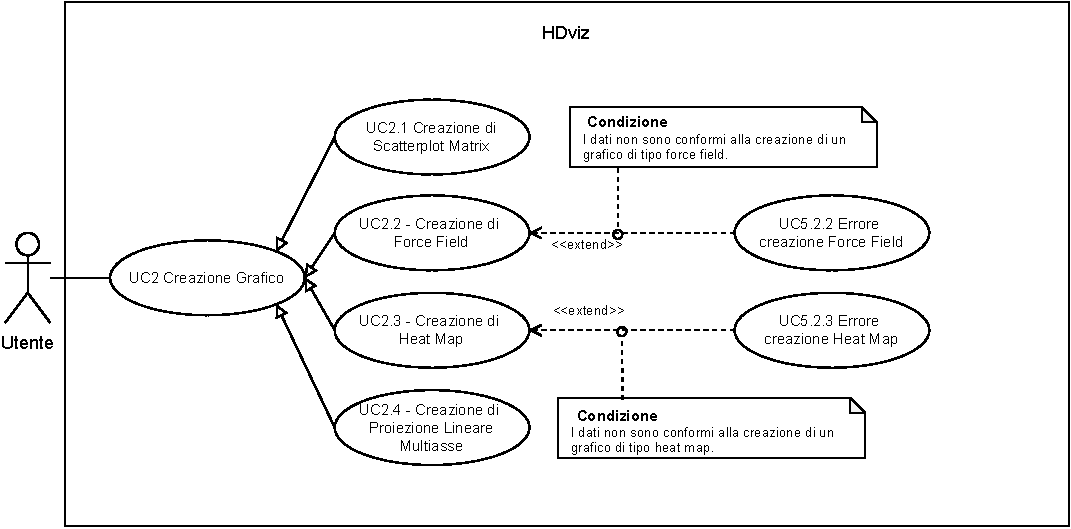
\includegraphics[width=0.8\textwidth]{componenti/casi-duso/diagrammi/UC2.pdf}
    \caption{Diagramma rappresentante UC2}
    \label{fig:UC4.4}
\end{figure}


\begin{itemize}
    \item \textbf{Descrizione}: L’utente vuole modificare la visualizzazione della Proiezione Lineare Multiasse
                                costruita dal dataset corrente.
	
    \item \textbf{Attore primario}: Utente.
    
    \item \textbf{Precondizione}:   La visualizzazione costruita dal dataset corrente è un grafico di tipo Proiezione Lineare Multiasse.
    \item \textbf{Postcondizione}:  Viene aggiornato il grafico costruito e visualizzato con i nuovi parametri.

	\item \textbf{Scenario principale}:
		\begin{enumerate}
            \item L'utente apporta le modifiche desiderate tra quelle offerte dalla Proiezione Lineare Multiasse.
        \end{enumerate}
\end{itemize}

\subsubsection{UC4.4.1 Aggiunta di una dimensione}
\label{subsec:uc4.2.1}
\begin{itemize}
    \item \textbf{Descrizione}: L’utente decide di visualizzare maggiori informazioni
                                aggiungendo una dimensione al grafico.

    \item \textbf{Attore primario}: Utente.
    
    \item \textbf{Precondizione}:   La visualizzazione costruita dal dataset corrente è una Proiezione Lineare Multiasse.
    \item \textbf{Postcondizione}:  La visualizzazione della PLA aggiunge una dimenisone.

	\item \textbf{Scenario principale}:
        \begin{enumerate}
            \item L'utente seleziona la voce "Dimensioni" e seleziona una dimensione da aggiungere alla proiezione.
            \item La visualizzazione aggiugne la dimensione selezionata e riposiziona i punti.
           
        \end{enumerate}
\end{itemize}

\subsubsection{UC4.4.2 Rimozione di una dimensione}
\label{subsec:uc4.2.1}
\begin{itemize}
    \item \textbf{Descrizione}: L’utente decide di rimuovere una dimensione dalla Proiezione Lineare Multiasse
                                a patto che essa non sia monodimensionale.

    \item \textbf{Attore primario}: Utente.
    
    \item \textbf{Precondizione}:   La visualizzazione costruita dal dataset corrente è una Proiezione Lineare Multiasse
                                    e rappresenta almeno due dimensioni.
    \item \textbf{Postcondizione}:  La visualizzazione della PLA rimuove una dimenisone.

	\item \textbf{Scenario principale}:
        \begin{enumerate}
            \item L'utente seleziona la voce "Dimensioni" e seleziona una dimensione da rimuovere dalla proiezione.
            \item La visualizzazione rimuove la dimensione selezionata e riposiziona i punti.
           
        \end{enumerate}
\end{itemize}


\subsubsection{UC4.4.2 Modifica proprietà dei punti per dimensione}
\label{subsec:uc4.2.1}
\begin{itemize}
    \item \textbf{Descrizione}: L’utente decide di manipolare la rappresentazione dei punti del grafico.

    \item \textbf{Attore primario}: Utente.
    
    \item \textbf{Precondizione}:   La visualizzazione costruita dal dataset corrente è una Proiezione Lineare Multiasse.
    \item \textbf{Postcondizione}:  La visualizzazione aggiorna i punti della PLA.

	\item \textbf{Scenario principale}:
        \begin{enumerate}
            \item L'utente seleziona la voce "Dimensioni-Proprietà" e seleziona una dimensione di cui modificare i punti.
            \item L'utente effettua le modifiche che desidera tra quelle proposte.
            \item La visualizzazione mostra i nuovi punti con le modifiche effettuate.
        \end{enumerate}
\end{itemize}


\subsubsection{UC4.4.2.1 Modifica colore}
\label{subsec:uc4.4.2.1}
\begin{itemize}
    \item \textbf{Descrizione}: L'utente decide di modificare il colore di punti relativi ad una dimensione.

	
    \item \textbf{Attore primario}: Utente.
    
    \item \textbf{Precondizione}:   L'utente ha selezionato l'opzione di modifica delle proprietà dei nodi per dimensione (UC4.4.2).
    \item \textbf{Postcondizione}:  Viene aggiornato il colore dei punti della dimensione selezionata.

	\item \textbf{Scenario principale}:
        \begin{enumerate}
            \item L'utente seleziona il nuovo colore da assegnare ai punti tra quelli resi disponbili.
        \end{enumerate}
\end{itemize}

\subsubsection{UC4.4.2.2 Modifica raggio}
\label{subsec:uc4.4.2.2}
\begin{itemize}
    \item \textbf{Descrizione}: L'utente decide di modificare il raggio di punti relativi ad una dimensione.
	
    \item \textbf{Attore primario}: Utente.
    
    \item \textbf{Precondizione}:   L'utente ha selezionato l'opzione di modifica delle proprietà dei punti per dimensione (UC4.4.2).
    \item \textbf{Postcondizione}:  Viene aggiornato il raggio dei punyi della dimensione selezionata.

	\item \textbf{Scenario principale}:
        \begin{enumerate}
            \item L'utente fa variare il raggio dei punti mediante uno slider.
        \end{enumerate}
\end{itemize}

\subsubsection{UC4.4.2.3 Modifica opacità}
\label{subsec:uc4.4.2.3}
\begin{itemize}
    \item \textbf{Descrizione}:  L'utente decide di modificare l'opacità dei punti relativi ad una dimensione.

	
    \item \textbf{Attore primario}: Utente.

    \item \textbf{Precondizione}: L'utente ha selezionato l'opzione di modifica delle proprietà dei punti per dimensione (UC4.4.2).
    \item \textbf{Postcondizione}:  Viene aggiornata l'opacità dei punti della dimensione selezionata.

	\item \textbf{Scenario principale}:
        \begin{enumerate}
            \item L'utente fa variare l'opacità dei punti mediante uno slider.
        \end{enumerate}
\end{itemize}


\subsection{UC4.5 Annulamento delle modifiche}

\begin{itemize}
    \item \textbf{Descrizione}: L'utente decide di scartare le modifiche fatte nella corrente selezione di modifica.

    \item \textbf{Attore primario}: Utente.
    
    \item \textbf{Precondizione}:   L'utente ha selezionato la voce di Modifica Grafico dal menu.
    \item \textbf{Postcondizione}:  Viene ripristinato il grafo ai parametri precedenti della selezione e visualizzato.

	\item \textbf{Scenario principale}:
        \begin{enumerate}

            \item L'utente seleziona il pulsante "Annulla modifiche".
            \item HDviz ripristina i parametri del grafo ai valori precedenti alla selezione del menu di modifica.
        
        \end{enumerate}
\end{itemize}




\newpage
\subsection{UC5 - Visualizzazione Errore}
\label{sub:uc5}

\begin{figure}[h]
    \centering
    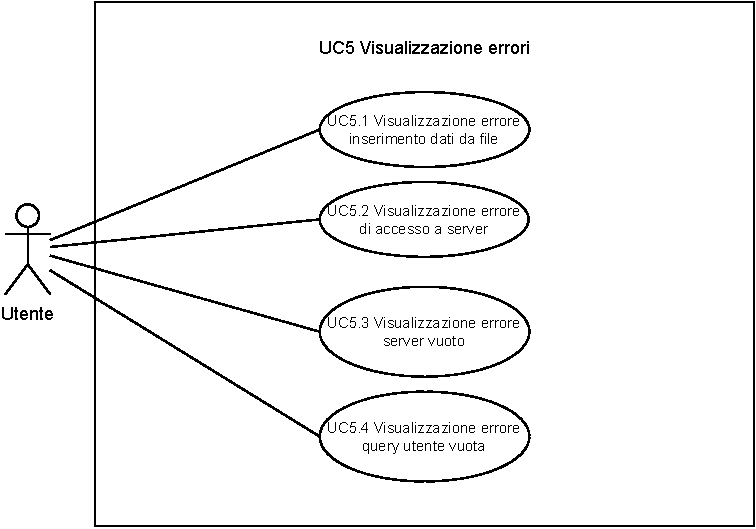
\includegraphics[width=0.7\textwidth]{componenti/casi-duso/diagrammi/UC5.pdf}
    \caption{Diagramma rappresentante UC5}
    \label{fig:UC5}
\end{figure}

\begin{itemize}
    \item \textbf{Descrizione}: Viene visualizzato un messaggio di errore relativo al fallimento di una specifica operazione.

    \item \textbf{Attore primario}: Utente.
    
    \item \textbf{Precondizione}:   Un'operazione fallisce

    \item \textbf{Postcondizione}:  Viene visualizzato un messaggio di errore.
    
    \item \textbf{Scenario Principale}:
    \begin{enumerate}
        \item Viene visualizzato il messaggio di errore.
        \item L'utente conferma di aver preso visione e viene reindirizzato alla home di HD Viz.
    \end{enumerate}

\end{itemize}

%TODO: Cambiare numerazione? Al momento ha senso da una parte ma non è giustificata qui visto che sottocasi non sono veri e propri.

\subsubsection{UC5.1 - Visualizzazione errore inserimento dati da file}
\label{ssub:uc5.1}
\begin{itemize}
    \item \textbf{Descrizione}: All'utente viene mostrato un messaggio d'errore al reperimento
                                dei dati dal file e continua ad utilizzare 
                                il software senza aver correttamente caricato un dataset valido.

    \item \textbf{Attore primario}: Utente.
    
    \item \textbf{Precondizione}:   Il caricamento di dati dal file.

    \item \textbf{Postcondizione}:  Viene visualizzato un messaggio di errore sul reperimento dei 
                                    dati che lo avvisa della mancata formazione di un dataset per il
                                    corretto utilizzo di HD Viz.

\end{itemize}


\subsubsection{UC5.2 - Visualizzazione errore di accesso a server}
\label{ssub:uc5.2}
\begin{itemize}
    \item \textbf{Descrizione}: All'utente viene mostrato un messaggio d'errore di accesso
                                al server al quale HD Viz si dovrebbe connettere, la creazione del dataset viene quindi interrotta.

    \item \textbf{Attore primario}: Utente.
    
    \item \textbf{Precondizione}:   L'apertura della connessione con il server fornito dall'utente fallisce.

    \item \textbf{Postcondizione}:  Viene visualizzato un messaggio di errore sull'apertura della connessione 
                                    con il server e della mancata formazione di un dataset per il corretto utilizzo di HD Viz.

\end{itemize}



\subsubsection{UC5.3 - Visualizzazione errore server vuoto}
\label{ssub:uc5.3}
\begin{itemize}
    \item \textbf{Descrizione}: Dopo aver aperto una connessione con un server HD Viz stabilisce non esserci
                                un database valido al reperimento dati per la creazione del dataset, la creazione
                                del dataset viene quindi interrotta.

    \item \textbf{Attore primario}: Utente.
    
    \item \textbf{Precondizione}:   Il server al quale HD Viz si è connesso è vuoto o i suoi database sono vuoti.

    \item \textbf{Postcondizione}:   Viene visualizzato un messaggio di errore sulla validità del server per il reperimento
                                    dei dati e della mancata formazione di un dataset per il corretto utilizzo di HD Viz.


\end{itemize}


\subsubsection{UC5.4 - Visualizzazione errore query utente vuota}
\label{ssub:uc5.4}
\begin{itemize}
    \item \textbf{Descrizione}: Messaggio relativo all'esecuzione di una query utente su server che restituisce 
                                un set di dati vuoto e
                                perciò la creazione del dataset risulta impossibile e viene interrotta.

    \item \textbf{Attore primario}: Utente.
    
    \item \textbf{Precondizione}:   La query eseguita su server restituisce un set di dati vuoto.

    \item \textbf{Postcondizione}:   Viene visualizzato un messaggio di errore sulla validità del risultato della query 
                                        in quanto vuota non permette la formazione di un dataset corretto per l'uso di HD Viz.


\end{itemize}

%TODO aggiungere altri casi d'uso

\end{document}